\section{Introduction}
Many high-stakes decisions rest on data that arrive one measurement at a time. 
A physician orders tests in sequence and uses signals from all the test results thus far to decide whether the next test is needed; an \textsc{mri} scanner fills in the $k$-space matrix line by line; a diffusion-weighted sequence in MR acquisition is repeated to raise its signal-to-noise ratio. 
In each case, every additional measurement costs time, money, or patient burden \citep{lustig2008compressed,zbontar2018fastmri}, so a sequential decision system faces two coupled questions: 1) \emph{what} to acquire next? and 2) \emph{when} enough has been acquired to stop safely?

% \begin{figure}[ht!]
%     \centering
%     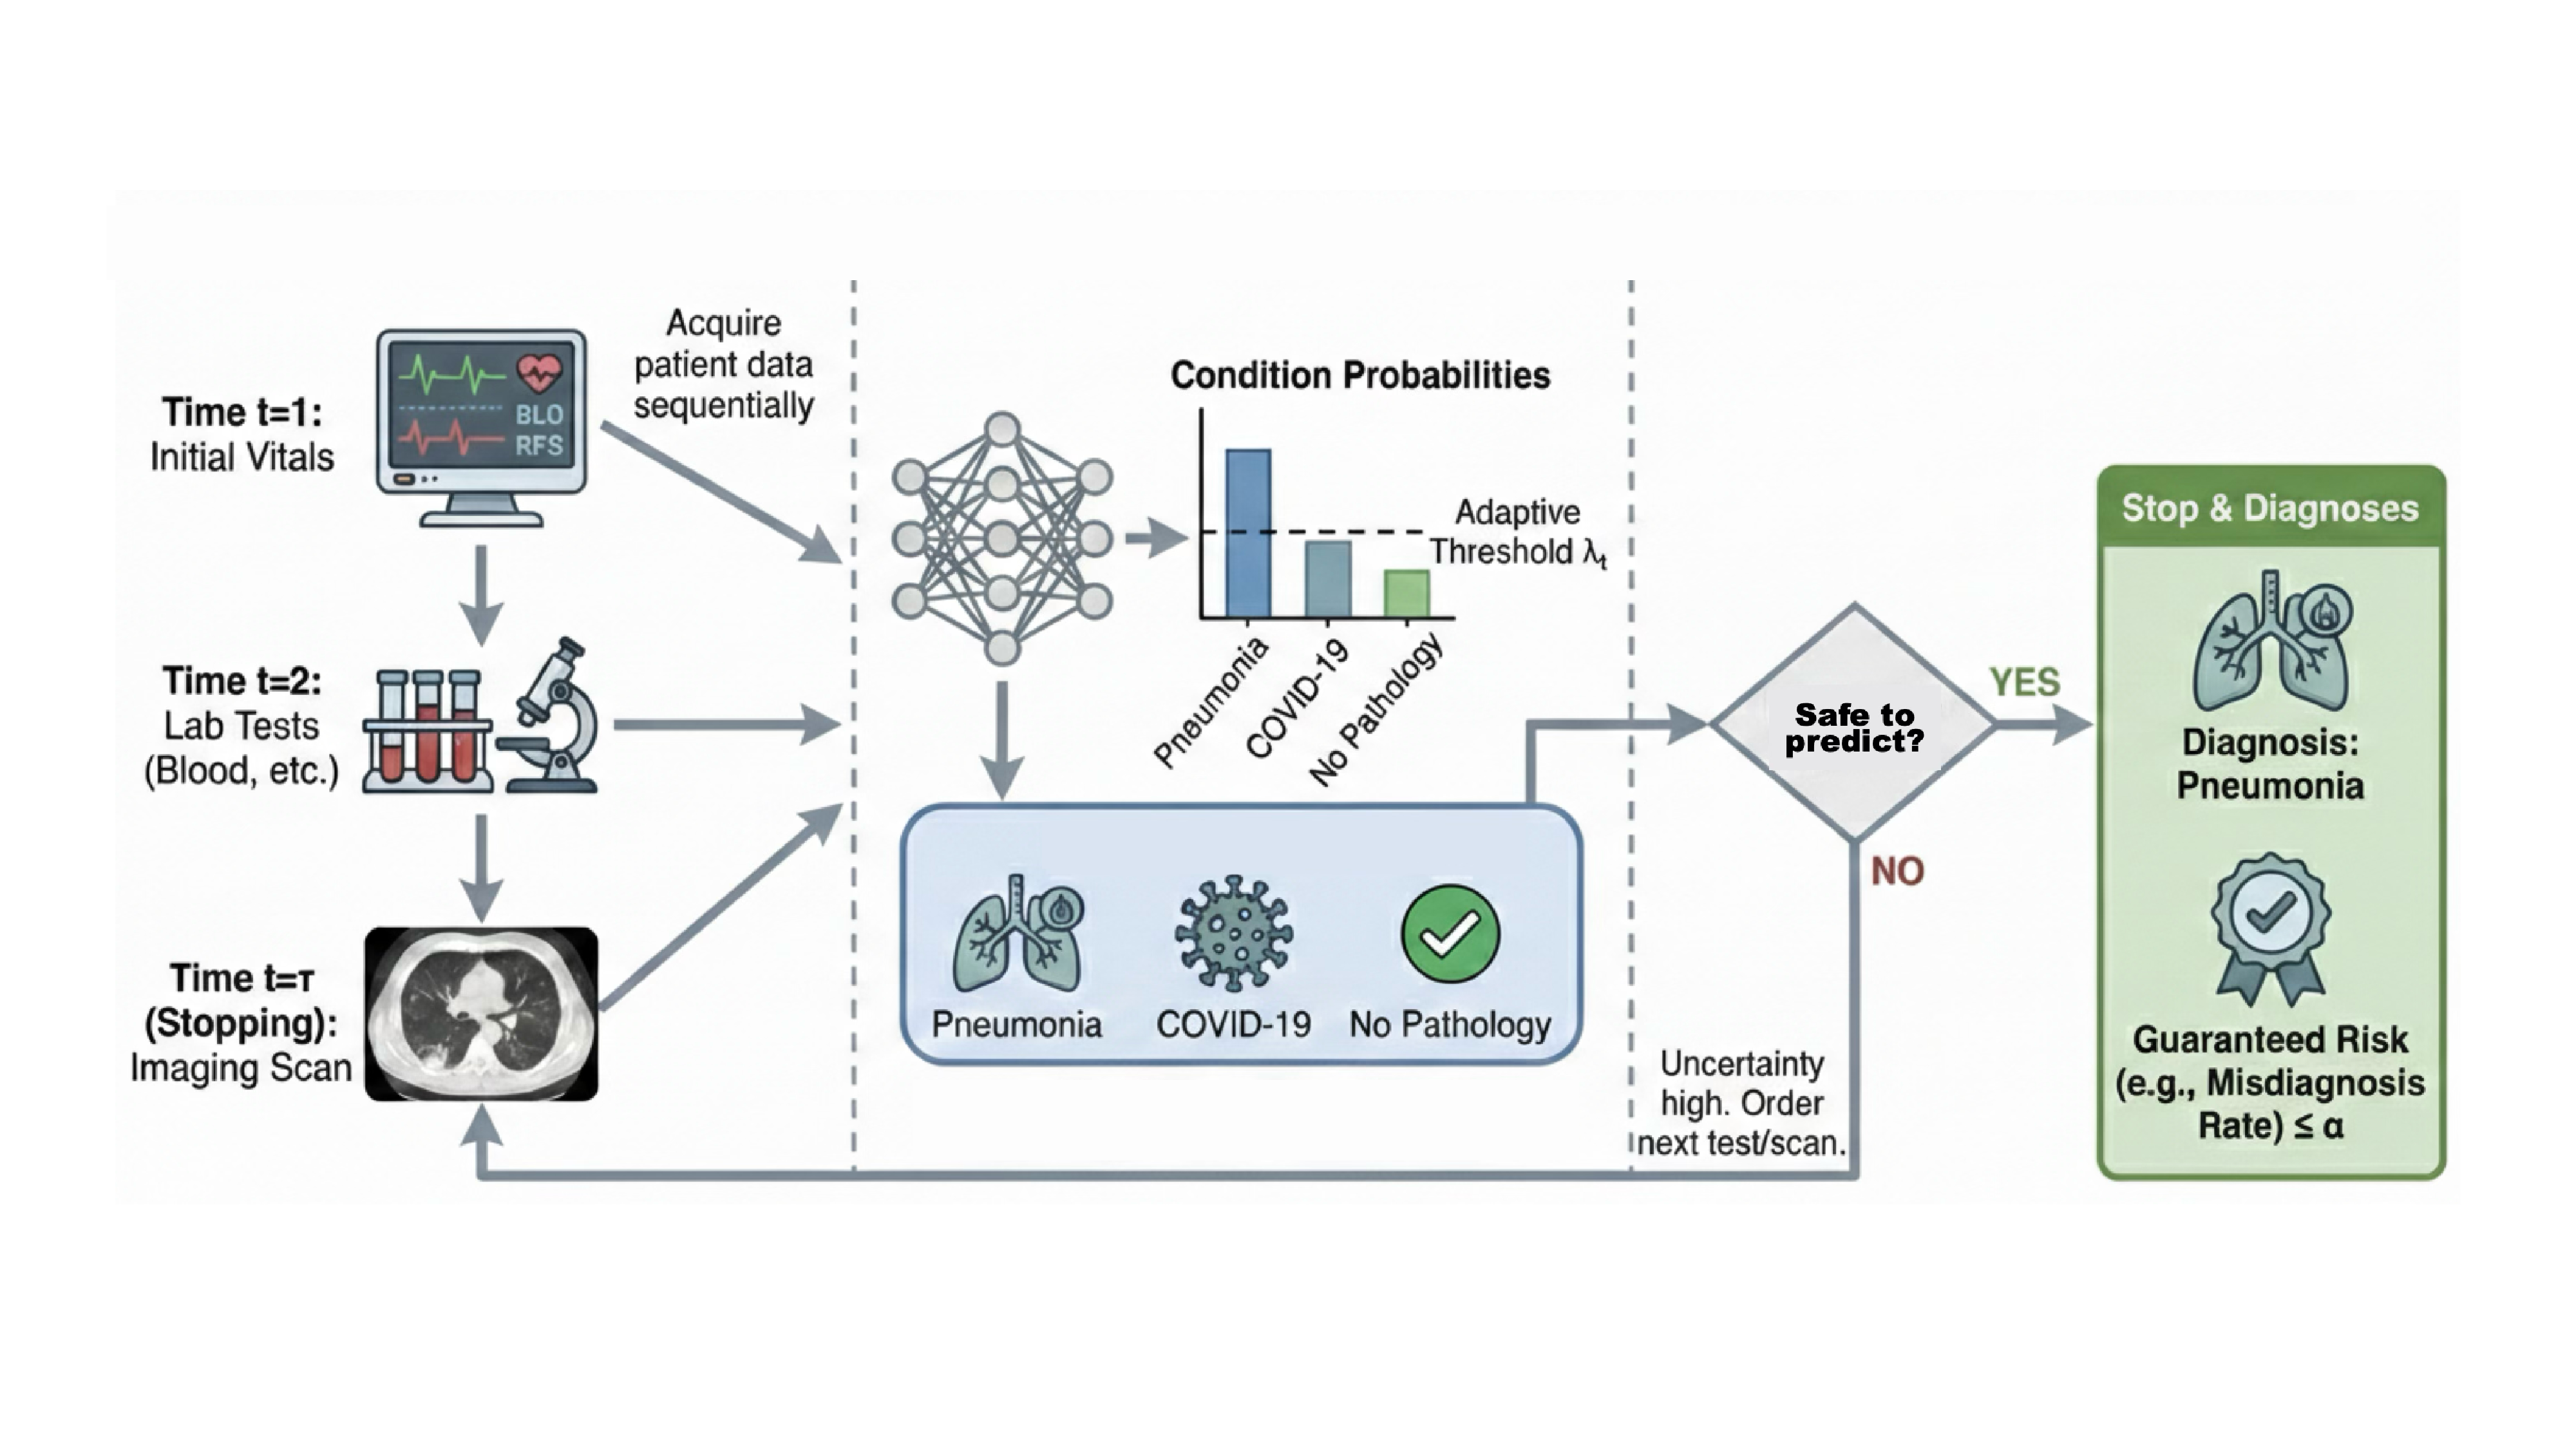
\includegraphics[width=0.8\linewidth]{figures/rcs_figure.pdf}
%     \vspace{-1cm}
%     \caption{\textbf{Risk-controlled stopping (\textsc{rcs}).} Data in clinical pipelines are acquired sequentially and each acquisition is costly. \gls{method} decides when to halt acquisition while guaranteeing that the risk of the resulting decision stays below a user-chosen level.}
%     \label{fig:rcs_figure}
% \end{figure}

The first question has received most of the attention. 
Dynamic feature acquisition methods learn policies that select informative measurements under a cost budget \citep{bakker2020experimental,singhal2023feasibility,covert2023learning,ASMR}. 
The second question is usually settled by a fixed budget, a confidence heuristic, or a learned policy tuned for average accuracy \citep{jafa-2018,bakker2020experimental}. 
None of these approaches offer a guarantee on the risk of the decision made when acquisition halts. 
This is consequential in safety-critical settings like healthcare, where stopping too early could produce unsafe decisions, and stopping too late wastes costs and increases patient burden.

We propose risk-controlled stopping (\textsc{rcs}), a post-hoc, distribution-free procedure for deciding when to stop acquisition so that a user-specified risk, such as misclassification, the false negative rate (\textsc{fnr}), or the false positive rate (\textsc{fpr}), stays below a chosen level. 
Two properties of the controlled risk set \gls{method} apart. 
First, it is an \emph{absolute} risk, measured against the ground-truth label rather than against the prediction the model would have made with all the data. 
Second, it is evaluated \emph{conditional on stopping}: only the samples on which the policy commits to a decision count. 
The second property is important, because a policy that rarely stops but is wrong on almost every sample where it stops can still satisfy a marginal risk bound over the full population.
Whereas a conditional risk bound rules out this behavior. 
%A marginal bound over the whole population is satisfied by a policy that stops rarely and errs on nearly everything it stops on; a conditional bound is not.

The statistical engine behind \gls{method} is the Learn-Then-Test (LTT) framework \citep{angelopoulos2025learn}, which certifies a family of parameterized predictors on a held-out calibration set with finite-sample, distribution-free guarantees. Our key observation is that a stopping rule is a form of selective predictor: it decides both \emph{whether} and \emph{when} to make a prediction, and thus on which partial observation the prediction is made. Treating each rule as a trajectory-level policy lets LTT certify the risk conditional on stopping directly. This guarantee comes from LTT and we do not claim a new bound or proof technique. 
%We are explicit that the certificate is inherited: \cref{thm:conditional_risk} is a corollary of LTT, and we claim no new bound or proof technique. 
Our contribution is the problem formulation, the definition of the risk being controlled, and the procedure needed to control it. 
An absolute risk admits no configuration that is safe by construction, so the set of certifiable rules can be non-monotone or empty. 
\gls{method} therefore calibrates with a step-down procedure rather than fixed-sequence testing, and when no rule can be certified with the available calibration data it defers to full acquisition rather than deploying an uncertified early-stopping policy.

We evaluate \gls{method} on one synthetic and two clinical tasks. The synthetic task, sequential patch acquisition on \textsc{CIFAR-10} \citep{cifar10}, validates the procedure under a controlled acquisition model. 
We draw no clinical conclusions from it. 
The clinical tasks use raw scanner measurements: slice-level abnormality detection from \textsc{fastMRI} knee $k$-space \citep{zbontar2018fastmri}, and PI-RADS-positive classification (radiologist-assigned PI-RADS $\geq 3$) from diffusion-weighted averages in an internal prostate \textsc{mri} cohort. 
Prior work has shown that a well-chosen subset of measurements can support reliable detection at a fixed undersampling factor \citep{singhal2023feasibility,ASMR}; it does not say when, for a given patient, acquisition can stop. \gls{method} answers that question with a certificate. The evaluated MRI checkpoints exhibit class-conditional \textsc{fnr} below the prescribed level; these stage-specific plots are empirical diagnostics, while the statistical certificate pertains to the eventually stopped cohort. The same procedure wraps a learned acquisition policy \citep{jafa-2018} without retraining.

\paragraph{Contributions}
\begin{itemize}[noitemsep]
    \item We propose \emph{risk-controlled stopping}: choosing when to halt sequential acquisition so that an absolute, user-specified risk against the ground-truth label (for example, \textsc{fnr}) is controlled on the samples the policy commits to. To our knowledge, no prior work casts acquisition stopping as a distribution-free, finite-sample risk-control problem.
    \item We show that treating each stopping rule as a trajectory-level selective policy makes this object certifiable by LTT (\cref{thm:conditional_risk} in Section \ref{sec:ltt}), and that the absolute-risk setting forces two design choices absent from relative-risk calibration: Holm's step-down without assuming an ordering of candidate risks, and explicit failure to certify when the certified set is empty, followed by an operational full-acquisition fallback.
    \item We instantiate the framework with class-conditional \textsc{fnr}/\textsc{fpr} and demonstrate certified control on scanner-ordered \textsc{mri} pipelines, on a synthetic \textsc{cifar}-10 benchmark, and as a post-hoc wrapper around a learned reinforcement-learning acquisition policy.
\end{itemize}
